% App. D figure: candidate features and quantile matching.
\begin{tikzpicture}[x=1cm,y=1cm]
\node[inner sep=0,anchor=north west] (tp) at (0,0)
  {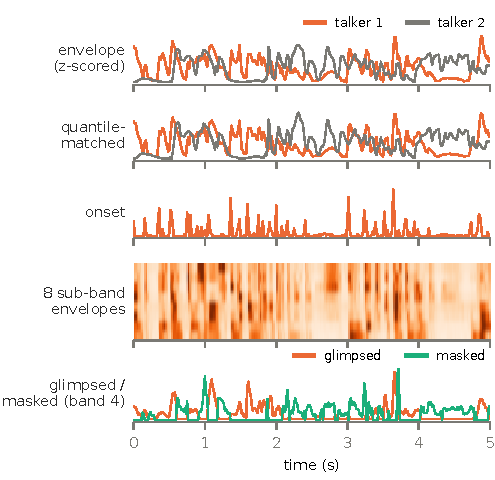
\includegraphics[width=7.2cm]{figures/net_feat_time.pdf}};
\node[ttl] at (0,0.25) {(a) one 5-s KU Leuven window, talker 1 attended};

% ---------------------------------------------------------------- (b) two branches
\def\px{8.1}
\node[ttl] at (\px,0.25) {(b) features of candidate $k$ in one window};
% broadband branch
\node[font=\scriptsize,anchor=west,text=cfInk,align=left] (bb) at (\px,-0.45) {broadband\\[-1pt]envelope};
\node[nbw={cfA}{1.25},minimum height=0.62cm,anchor=west] (z1) at (\px+1.8,-0.45) {z-score};
\node[nbw={cfA}{1.75},minimum height=0.62cm,anchor=west] (qm) at ($(z1.east)+(0.3,0)$)
  {quantile-match\\[-1pt]across $k$};
\node[nbw={cfA}{1.3},minimum height=0.62cm,anchor=west] (on) at ($(qm.east)+(0.3,0)$)
  {onset\\[-1pt]$\max(0,\Delta)$};
\draw[ar=cfA] (bb) -- (z1);
\draw[ar=cfA] (z1) -- (qm);
\draw[ar=cfA] (qm) -- (on);
% sub-band branch
\node[font=\scriptsize,anchor=west,text=cfInk,align=left] (sb) at (\px,-1.45) {8 + 28 sub-\\[-1pt]band env.};
\node[nbw={cfA}{1.25},minimum height=0.62cm,anchor=west] (z2) at (\px+1.8,-1.45) {z-score};
\node[nbw={cfC}{3.35},minimum height=0.62cm,anchor=west] (gl) at ($(z2.east)+(0.3,0)$)
  {8 bands: glimpsed / masked where\\[-1pt]$a_k\ge$ / $<\max_{j\ne k}a_j$};
\draw[ar=cfA] (sb) -- (z2);
\draw[ar=cfA] (z2) -- (gl);

% ---------------------------------------------------------------- channel stack
\def\u{0.112}
\def\sy{-2.95}
\coordinate (c0) at (\px,\sy);
\foreach \w/\c/\lab [count=\i] in
  {1/cfA!80/{}, 1/cfA!55/{}, 8/cfA!35/{8}, 28/cfA!18/{28}, 8/cfC!50/{8}, 8/cfC!22/{8}} {
  \ifnum\i=1 \coordinate (L\i) at (c0); \else
    \pgfmathtruncatemacro{\j}{\i-1}\coordinate (L\i) at (R\j); \fi
  \coordinate (R\i) at ($(L\i)+(\w*\u,0)$);
  \fill[\c] (L\i) rectangle ($(R\i)+(0,0.5)$);
  \draw[white,line width=0.8pt] (R\i) -- ++(0,0.5);
  \node[font=\tiny,text=cfInk] at ($(L\i)!0.5!(R\i)+(0,0.25)$) {\lab};
}
\draw[ar=cfInk] ($(L1)!0.5!(R6)+(0,1.02)$) -- ($(L1)!0.5!(R6)+(0,0.55)$)
  node[arl,pos=0.45,right=1pt] {concatenate};
\draw[decorate,decoration={brace,amplitude=3pt,mirror},cfInk,line width=0.4pt]
  ($(L1)+(0,-0.06)$) -- ($(R6)+(0,-0.06)$) node[midway,below=3pt,font=\scriptsize]
  {54 channels $\times\,L'$ per candidate $\to$ shared audio encoder};
% key
\foreach \c/\lab [count=\i] in {cfA!80/envelope (matched), cfA!55/onset (matched),
  cfA!35/8 sub-bands, cfA!18/28 sub-bands, cfC!50/glimpsed, cfC!22/masked} {
  \pgfmathsetmacro{\kx}{\px+mod(\i-1,2)*2.6}
  \pgfmathsetmacro{\ky}{\sy-0.95-floor((\i-1)/2)*0.26}
  \fill[\c] (\kx,\ky) rectangle ++(0.22,0.15);
  \node[font=\tiny,anchor=west,text=cfInk] at (\kx+0.24,\ky+0.075) {\lab};
}

% ---------------------------------------------------------------- (c) histograms
\node[ttl] at (\px,-4.85) {(c) value distributions in the window};
\node[inner sep=0,anchor=north west] (hi) at (\px,-5.05)
  {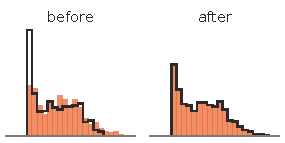
\includegraphics[width=3.3cm]{figures/net_feat_hist.pdf}};
\node[note,anchor=north west,text width=2.9cm] at ($(hi.north east)+(0.15,0)$)
  {After matching both candidates have the same values, so level and loudness no longer
   mark a talker; each keeps its own time course (a).};
\end{tikzpicture}
